\documentclass[10pt]{article}
\usepackage[utf8]{inputenc}
\usepackage[T1,T2A]{fontenc}
\usepackage{hyperref}
\hypersetup{colorlinks=true, linkcolor=black, filecolor=magenta, urlcolor=cyan,}
\urlstyle{same}
\usepackage{amsmath}
\usepackage{amsfonts}
\usepackage{amssymb}
\usepackage[version=4]{mhchem}
\usepackage{stmaryrd}
\usepackage{bbold}
\usepackage{graphicx}
\usepackage[export]{adjustbox}

\usepackage{mathtools}
\usepackage{makecell}
\usepackage{parskip}

\usepackage[margin=2cm]{geometry}
\usepackage{tikz}
\usepackage{enumitem}

\graphicspath{ {notes-09-transformer} }

\newcommand{\verteq}{\rotatebox{90}{$\,=$}}
\newcommand{\equalto}[2]{\underset{\scriptstyle\overset{\mkern4mu\verteq}{#2}}{#1}}

\begin{document}

\begin{center}
    \Huge{Deep Learning: Attention, Transformer}
    
    \vspace{0.5cm}
    \huge{Lecture 09.12}

    \vspace{0.5cm}
    \large \href{https://t.me/foma2u}{Foma Shipilov}
\end{center}


\tableofcontents
\newpage

\section*{Language Models}

\subsection*{Autoregressive Modelling}

The joint probability of a sequence is factored into a product of conditionals:

\begin{equation*} 
p(x)=p(x_1) p(x_2 | x_1) p(x_3 | x_1, x_2) \ldots p (x_{T} | x_{1}\ldots x_{T-1})
\end{equation*}

Generation starts from $\langle\text{BOS}\rangle$ and proceeds step by step --- 
at each step a token is sampled and fed back into the model:

\begin{equation*} 
\langle\text{BOS}\rangle \rightarrow \text{RNN} \rightarrow \text{Linear} 
\rightarrow \text{Logits} \in \mathbb{R}^{|v|} \rightarrow \text{softmax} 
\rightarrow p (x | x_{0}= \langle\text{BOS}\rangle)
\end{equation*}
\begin{equation*} 
\text{sample}\quad x_1 \rightarrow \text{RNN} \rightarrow \text{Linear} 
\rightarrow \text{Logits} \rightarrow p (x | x_{0}= \langle\text{BOS}\rangle, x_1 = x_1)
\end{equation*}
\begin{equation*} 
\text{sample}\quad x_2 \rightarrow \text{RNN} \rightarrow \text{Linear} 
\rightarrow \text{Logits} \rightarrow p (x | x_{0}= \langle\text{BOS}\rangle, x_1 = x_1)
\end{equation*}

Until $\langle\text{EOS}\rangle$ --- End of Sequence.

\section*{Training a Language Model}

Let $\theta$ be the model parameters, $X=(x_1, \ldots, x_{T})$ a real sequence.
Training minimizes the negative log-likelihood:

\begin{equation*} 
p_{\theta} (x) = \equalto{p_{\theta} (x_0)}{1} p_{\theta} (x_1 | x_0) \ldots 
p(x_{T} | x_{0}, x_{1}, \ldots, x_{T-1})
\end{equation*}

\begin{equation*} 
-\sum_{t=1}^{T} \log p_{\theta} (x_{t} | x_{0}, \ldots, x_{t-1}) \rightarrow \min
\end{equation*}

\section{Attention, Transformer}

\subsection{Attention Layers}


\subsubsection{Previous architectures}

Before attention mechanisms were introduced, three main types of layers 
were used to process sequences, each with significant drawbacks:
\begin{center}
\renewcommand{\arraystretch}{1.1}
\begin{tabular}{|p{4cm}|p{4cm}|p{4cm}|}
\hline
\rule{0pt}{10pt}\textbf{Fully-connected} & \textbf{Convolutional} & \textbf{Recurrent} \\
\hline
\rule{0pt}{8pt}
\textit{Problems:}
\begin{itemize}[leftmargin=*, topsep=2pt]
    \item Fixed window
    \item A lot of weights
\end{itemize} &
\textit{Problems:}
\begin{itemize}[leftmargin=*, topsep=2pt]
    \item Local dependencies only
\end{itemize} &
\textit{Problems:}
\begin{itemize}[leftmargin=*, topsep=2pt]
    \item Slow training
    \item Troubles with gradients
\end{itemize} \\
\hline
\end{tabular}
\end{center}


\subsubsection{Attention layer}

Unlike previous architectures, the attention layer processes all tokens simultaneously.
For each output, the model dynamically computes how relevant every input token is
and takes a weighted sum --- tokens that matter more get higher weights.
\begin{center}
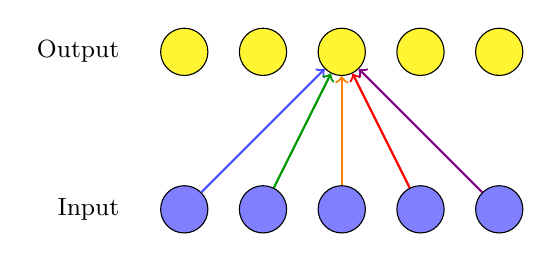
\begin{tikzpicture}
    \foreach \x in {0,1,2,3,4} {
        \node[circle, draw, fill=blue!50, minimum size=0.6cm] (b\x) at (\x, 0) {};
    }
    \foreach \x in {0,1,2,3,4} {
        \node[circle, draw, fill=yellow!80, minimum size=0.6cm] (t\x) at (\x, 2) {};
    }
    \draw[->, thick, blue!70] (b0) -- (t2);
    \draw[->, thick, green!60!black] (b1) -- (t2);
    \draw[->, thick, orange] (b2) -- (t2);
    \draw[->, thick, red] (b3) -- (t2);
    \draw[->, thick, violet] (b4) -- (t2);
    \node[left] at (-0.7, 0) {\small Input};
    \node[left] at (-0.7, 2) {\small Output};
\end{tikzpicture}
\end{center}

The attention layer addresses all the limitations of previous architectures:
\begin{itemize}
    \item Look at all inputs to learn more global dependencies
    \item Share weights to work with variable length window
    \item Do not use autoregressive structure to make training parallelizable
\end{itemize}

\subsubsection{Self-attention: idea}

Each token embedding is updated using information from all other tokens in the sequence.
So for each token, the model does two things:
\begin{itemize}
    \item Find tokens relevant to the current one (compute relevance scores)
    \item Compute the weighted combination of their embeddings
\end{itemize}

Relevance scores are dot products of queries and keys, normalized via softmax:

\begin{equation*} 
p = \text{softmax}(k_{1}^{T} q_{i},\ k_{2}^{T} q_{i},\ \ldots,\ k_{l}^{T} q_{i})
\end{equation*}

The updated embedding is a weighted sum of value vectors:

\begin{equation*} 
\tilde{x}_{i} = \sum\limits_{j=1}^{L} p_{j} \cdot V_{j}
\end{equation*}

where $q_i$ --- query for token $i$ (what this token is looking for),\quad
$k_j$ --- key for token $j$ (what it has to offer),\quad
$V_j$ --- value for token $j$ (what it actually contains).


\subsubsection{Self-attention}

\begin{minipage}{0.6\textwidth}
Now we can write the same operation in matrix form for all tokens simultaneously.
To compute relevance scores we use two linear transformations of the input: 

\begin{equation*}
Q = XW^Q, \quad K = XW^K
\end{equation*}

And to compute final embeddings we use the third one - V - values:

\begin{equation*}
\quad V = XW^V
\end{equation*}

where $Q, K, V \in \mathbb{R}^{L \times d}$. The attention output is then:

\begin{equation*}
\text{Attention}(Q, K, V) = \text{softmax} \left(\frac{QK^{T}}{\sqrt{d_{k}}}\right) V
\end{equation*}

$X \in \mathbb{R}^{L \times d}\rightarrow A = QK^{T} \in \mathbb{R}^{L \times L}$ --- is the attention matrix (entry $(i,j)$ reflects how relevant token $j$ is to token $i$).

*Dividing by $\sqrt{d_k}$ prevents 
the dot products from growing too large before softmax.
\end{minipage}
\hfill
\begin{minipage}{0.35\textwidth}
    \centering
    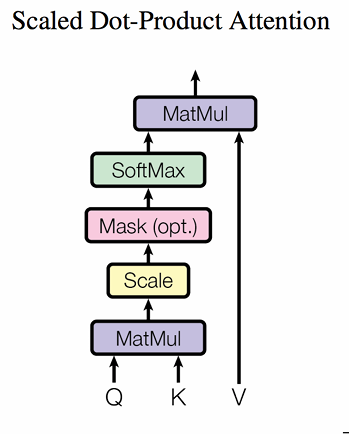
\includegraphics[width=0.8\textwidth]{attention_scheme.png}
\end{minipage}


\subsubsection{Self-attention step by step}

\textbf{Step 1.} Compute queries, keys, values for all inputs
using the same linear transformations:

\begin{equation*}
q_{i} = x_{i} W^{Q}, \qquad k_{i} = x_{i} W^{K}, \qquad v_{i} = x_{i} W^{V}
\end{equation*}

\textbf{Step 2.} For token $i$, compute relevance scores using
query $i$ and all the keys, then normalize via softmax:

Consider an example: We have two input tokens ---
``Thinking'' and ``Machines''. Each embedding has 4 dimensions,
each query/key/value vector has 4 dimensions, $d_k = 64$, so $\sqrt{d_k} = 8$.

\begin{center}
\renewcommand{\arraystretch}{1.1}
\begin{tabular}{|p{4.5cm}|>{\centering\arraybackslash}p{4.5cm}|>{\centering\arraybackslash}p{4.5cm}|}
\hline
\rule{0pt}{10pt}\textbf{Operation} & \textbf{Token 1} & \textbf{Token 2} \\
\hline
\rule{0pt}{8pt}Input & ``Thinking'' & ``Machines'' \\
\hline
Embedding $x_i$ & $x_1$ & $x_2$ \\
\hline
Query $q_i = x_i W^Q$ & $q_1$ & $q_2$ \\
\hline
Key $k_i = x_i W^K$ & $k_1$ & $k_2$ \\
\hline
Value $v_i = x_i W^V$ & $v_1$ & $v_2$ \\
\hline
Score $q_1 \cdot k_j^T$ & $q_1 \cdot k_1 = 112$ & $q_1 \cdot k_2 = 96$ \\
\hline
Scale $/ \sqrt{d_k}$ (= 8) & $112 / 8 = 14$ & $96 / 8 = 12$ \\
\hline
Softmax & $0.88$ & $0.12$ \\
\hline
Weighted sum & \multicolumn{2}{c|}{$z_1 = 0.88 \cdot v_1 + 0.12 \cdot v_2$} \\
\hline
\end{tabular}
\end{center}

Token 1 attends mostly to itself --- its weight 0.88 is significantly
higher than the weight of token 2.

\textbf{Step 3.} Compute weighted combination of values,
weights from relevance scores:

\begin{equation*}
z_1 = 0.88 \cdot v_1 + 0.12 \cdot v_2
\end{equation*}

$z_1$ is the new embedding of token 1 --- now it knows about all other tokens in the sequence.


\subsubsection{Self-attention in matrix form}

All operations from the 1.1.5 can be written compactly in matrix form.
$Q$, $K$, $V$ are obtained via linear projections of the input matrix $X$:

\textbf{Step 1.} Project input into $Q$, $K$, $V$:

\begin{equation*}
X \times W^{Q} = Q, \qquad X \times W^{K} = K, \qquad X \times W^{V} = V
\end{equation*}

Each row of $Q$, $K$, $V$ corresponds to one token.

\textbf{Step 2.} Compute attention output $Z$:

\begin{equation*}
Z = \text{Attention}(Q, K, V) = \text{softmax} \left(\frac{Q \times K^{T}}{\sqrt{d_{k}}}\right) V
\end{equation*}

\begin{equation*}
QK^T \xrightarrow{\text{gives}} \text{relevance scores for all token pairs}
\xrightarrow{/\sqrt{d_k}} \text{scale}
\xrightarrow{\text{softmax}} \text{weights}
\xrightarrow{\times V} Z
\end{equation*}


\subsubsection{Attention matrix}

The result of $\text{softmax}\left(\frac{QK^T}{\sqrt{d_k}}\right)$
is an $L \times L$ matrix where entry $(i,j)$ is the attention
weight of token $i$ towards token $j$. Each row sums to 1.

\begin{center}
    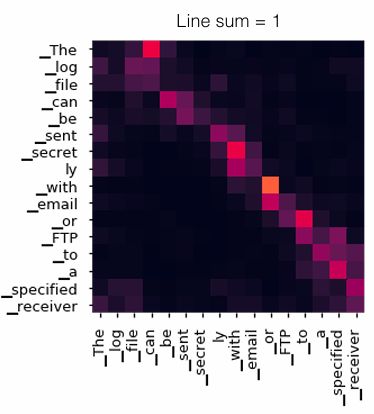
\includegraphics[width=0.3\textwidth]{attention_matrix.png}
\end{center}


\subsubsection{Other score functions}

\begin{center}
\renewcommand{\arraystretch}{1.5}
\begin{tabular}{|m{2.3cm}|m{10cm}|m{2.3cm}|}
\hline
\rule{0pt}{10pt}\textbf{Name} & \textbf{Alignment score function} & \textbf{Citation} \\
\hline
\rule{0pt}{8pt}Content-base attention & $\operatorname{score}\left(s_t, \boldsymbol{h}_i\right)=\operatorname{cosine}\left[s_t, \boldsymbol{h}_i\right]$ & Graves2014 \\
\hline
Additive(*) & $\operatorname{score}\left(\boldsymbol{s}_t, \boldsymbol{h}_i\right)=\mathbf{v}_a^{T} \tanh \left(\mathbf{W}_a\left[\boldsymbol{s}_t ; \boldsymbol{h}_i\right]\right)$ & Bahdanau2015 \\
\hline
Location-Base & $\alpha_{t, i}=\text{softmax}\left(\mathbf{W}_a \boldsymbol{s}_t\right)$

\textit{Note: This simplifies the softmax alignment to only depend on the target position.} & Luong2015 \\
\hline
General & $\operatorname{score}\left(s_t, \boldsymbol{h}_i\right)=s_t^{T} \mathbf{W}_a \boldsymbol{h}_i$

where $\mathbf{W}_a$ is a trainable weight matrix in the attention layer & Luong2015 \\
\hline
Dot-Product & $\operatorname{score}\left(\boldsymbol{s}_t, \boldsymbol{h}_i\right)=\boldsymbol{s}_t^{T} \boldsymbol{h}_i$ & Luong2015 \\
\hline
Scaled Dot-Product($\wedge$) & $\operatorname{score}\left(s_t, h_i\right)=\frac{s_i^{T} h_i}{\sqrt{n}}$

\textit{Note: very similar to the dot-product attention except for a scaling factor; where n is the dimension of the source hidden state.} & Vaswani2017 \\
\hline
\end{tabular}
\end{center}

\subsubsection{Complexity}

$L \rightarrow n$

Table 1: Maximum path lengths, per--layer complexity and minimum number of sequential operations for different layer types, \textit{n} is the sequence length, \textit{d} is the representation dimension, \textit{k} is the kernel size of convolutions and \textit{r} --- the size of the neighborhood in restricted self---attention.

\begin{center}
\renewcommand{\arraystretch}{1.5}
\begin{tabular}{|m{4.5cm}|m{3cm}|m{3cm}|m{3cm}|}
\hline
\rule{0pt}{10pt}\textbf{Layer Type} & \textbf{Complexity per Layer} & \textbf{Sequential Operations} & \textbf{Maximum Path Length} \\
\hline
\rule{0pt}{8pt}Self-Attention & $O(n^{2} \cdot d)$ & $O(1)$ & $O(1)$ \\
\hline
Recurrent & $O(n \cdot d^{2})$ & $O(n)$ & $O(n)$ \\
\hline
Convolutional & $O(k \cdot n \cdot d^{2})$ & $O(1)$ & $O(\log_{k}(n))$ \\
\hline
Self-Attention (restricted) & $O(r \cdot n \cdot d)$ & $O(1)$ & $O(n/r)$ \\
\hline
\end{tabular}
\end{center}
Self-Attention is the most parallelizable and captures long-range dependencies in a single step. The downside is $O(n^2 \cdot d)$ complexity --- the longer
the sequence, the more expensive it gets. \textbf{Restricted self-attention} reduces complexity to $O(r \cdot n \cdot d)$ by limiting each token to only $r$ neighbors, at the cost of losing global context.


\subsubsection{Multi-Head Attention: idea}

A single attention head learns one type of relevance.
But language has many different types of dependencies simultaneously ---
syntactic, semantic, coreference, and others.

That is why Multi-Head Attention was introduced --- it runs $h$ attention heads in parallel, each learning its own type of relevance. The outputs are then concatenated:

\begin{itemize}
    \item \textbf{Single-head attention} --- one relevance pattern for all tokens
    \item \textbf{Multi-head attention} --- $h$ different relevance patterns,
    each capturing a different type of relevance
\end{itemize}


\subsubsection{Multi-Head Attention}

\begin{minipage}{0.6\textwidth}
Each head has its own projection matrices and learns
its own type of relevance:

\begin{equation*}
\operatorname{head}_{i} = \text{Attention}(QW_{i}^{Q},\ KW_{i}^{K},\ VW_{i}^{V})
\end{equation*}

The outputs are concatenated and projected back:

\begin{equation*}
\text{MultiHead}(Q, K, V) = \text{Concat}(\operatorname{head}_{1}, \ldots, \operatorname{head}_{h})\, W^{0}
\end{equation*}
\end{minipage}
\hfill
\begin{minipage}{0.35\textwidth}
    \centering
    \includegraphics[width=0.7\textwidth]{multihead.png}
\end{minipage}


\subsubsection{Multi-Head Attention: step by step}

\textbf{Step 1.} Take the input sentence.

\textbf{Step 2.} We embed each word.*

\textbf{Step 3.} Split into 8 heads. We multiply $X$ or $R$ with weight matrices
to get $Q_i$, $K_i$, $V_i$ for each head.

\textbf{Step 4.} Calculate attention using the resulting $Q$/$K$/$V$ matrices.

\textbf{Step 5.} Concatenate the resulting $Z$ matrices, then multiply with weight matrix $W^{0}$ to produce the output of the layer.

\vspace{0.3cm}
* In all encoders other than N0, we don't need embedding. We start directly with the output of the encoder right below this one


\subsubsection{Multi-Head Attention: trainable parameters}

\begin{equation*}
\text{MultiHead}(Q, K, V) = \text{Concat}(\operatorname{head}_{1}, \ldots, \operatorname{head}_{h})\, W^{0}
\end{equation*}
\begin{equation*}
\operatorname{head}_{i} = \text{Attention}(QW_{i}^{Q},\ KW_{i}^{K},\ VW_{i}^{V})
\end{equation*}

Each head has its own set of projection matrices.
Their dimensions are chosen so that the total computation stays comparable to single-head attention:

\begin{equation*}
W_{i}^{Q} \in \mathbb{R}^{d_{\text{model}} \times d_{k}}, \quad
W_{i}^{K} \in \mathbb{R}^{d_{\text{model}} \times d_{k}}, \quad
W_{i}^{V} \in \mathbb{R}^{d_{\text{model}} \times d_{v}}
\end{equation*}

\begin{equation*}
W^{0} \in \mathbb{R}^{h d_{v} \times d_{\text{model}}}
\end{equation*}

where $d_k = d_v = d_{\text{model}} / h$ --- each head works in a lower-dimensional space $d^{\prime} = \frac{d}{h}$, but all $h$ heads together
cover the full dimensionality $d_{\text{model}}$.

$h$ --- num heads


\newpage
\subsection{Transformer Model}

\subsubsection{Transformer model overview}

The Transformer was originally proposed for neural machine translation --- a seq2seq task where the input and output are sequences of different lengths.

\begin{itemize}
    \item Encoder--decoder architecture
    \item 3 types of attention operators:
    \begin{itemize}
        \item \textbf {Encoder--encoder} (self--attention):tokens of the input sequence attend to each other to build context-aware representations.
        \item \textbf {Decoder--decoder} (self--attention): each token can only attend to previous tokens, not future ones.
        \item \textbf {Encoder--decoder}: the decoder attends to the encoder output to find relevant information from the input sequence.
    \end{itemize}
    \item Other operations (position--wise):
    \begin{itemize}
        \item \textbf {Feed forward layers}
        \item \textbf {Residual connections}: help gradients flow through deep networks
        \item \textbf {Layer norm}: stabilizes training
    \end{itemize}
    \item \textbf {Positional encoding}: position information is added to the embeddings
\end{itemize}

\subsubsection{Encoder--encoder attention}

\begin{center}
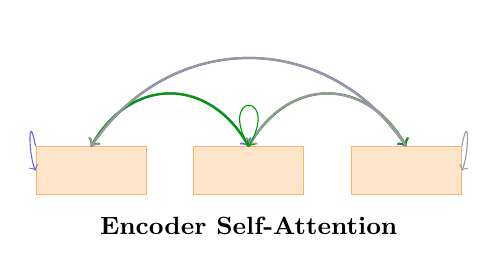
\begin{tikzpicture}
    % три токена
    \foreach \x in {0, 2, 4} {
        \node[rectangle, draw=orange!60, fill=orange!20,
              minimum width=1.4cm, minimum height=0.6cm]
              (t\x) at (\x, 0) {};
    }

    % стрелки от каждого к каждому
    \draw[->, blue!60, thick] (t0.north) 
        .. controls (0.5, 1.2) and (1.5, 1.2) .. (t2.north);
    \draw[->, blue!60, thick] (t0.north) 
        .. controls (1, 1.8) and (3, 1.8) .. (t4.north);
    \draw[->, green!60!black, thick] (t2.north) 
        .. controls (1.5, 1.2) and (0.5, 1.2) .. (t0.north);
    \draw[->, green!60!black, thick] (t2.north) 
        .. controls (2.5, 1.2) and (3.5, 1.2) .. (t4.north);
    \draw[->, gray!80, thick] (t4.north) 
        .. controls (3.5, 1.2) and (2.5, 1.2) .. (t2.north);
    \draw[->, gray!80, thick] (t4.north) 
        .. controls (3, 1.8) and (1, 1.8) .. (t0.north);

    % стрелки на себя
    \draw[->, blue!60] (t0.north west) 
        .. controls (-0.8, 0.8) and (-0.8, 0.2) .. (t0.west);
    \draw[->, green!60!black] (t2.north) 
        .. controls (1.6, 1.0) and (2.4, 1.0) .. (t2.north);
    \draw[->, gray!80] (t4.north east) 
        .. controls (4.8, 0.8) and (4.8, 0.2) .. (t4.east);

    \node[font=\small\bfseries] at (2, -0.7) {Encoder Self-Attention};
\end{tikzpicture}
\end{center}

The one we have discussed earlier:
\begin{itemize}
    \item Multi--head
    \item Scaled dot--product
    \item  Self--attention: Q, K, V are computed from the same input matrix X
\end{itemize}

Update embeddings of tokens from the input sequence


\subsubsection{Decoder--decoder attention}

\begin{center}
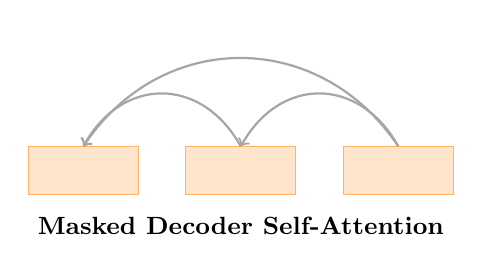
\begin{tikzpicture}
    % три токена
    \foreach \x in {0, 2, 4} {
        \node[rectangle, draw=orange!60, fill=orange!20,
              minimum width=1.4cm, minimum height=0.6cm]
              (t\x) at (\x, 0) {};
    }

    % токен 2 смотрит на токен 1
    \draw[->, gray!70, thick] (t2.north)
        .. controls (1.5, 1.2) and (0.5, 1.2) .. (t0.north);

    % токен 3 смотрит на токен 1 и токен 2
    \draw[->, gray!70, thick] (t4.north)
        .. controls (3.5, 1.2) and (2.5, 1.2) .. (t2.north);
    \draw[->, gray!70, thick] (t4.north)
        .. controls (3, 1.8) and (1, 1.8) .. (t0.north);

    \node[font=\small\bfseries] at (2, -0.7) {Masked Decoder Self-Attention};
\end{tikzpicture}
\end{center}

During training, the decoder must not look at future tokens. This is achieved by masking the attention matrix:

\begin{equation*}
W_{ij}^{\prime} \longleftarrow -\infty \quad \text{if } j > i
\end{equation*}

Setting future positions to $-\infty$ before softmax makes their attention weights effectively zero:

\begin{equation*}
W = \operatorname{softmax}(W^{\prime})
\end{equation*}

Each token can only attend to previous tokens in the generated sequence.


\subsubsection{Encoder--decoder attention}

\begin{center}
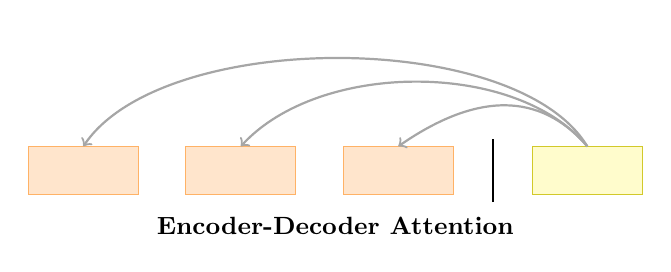
\begin{tikzpicture}
    % три токена энкодера
    \foreach \x in {0, 2, 4} {
        \node[rectangle, draw=orange!60, fill=orange!20,
              minimum width=1.4cm, minimum height=0.6cm]
              (e\x) at (\x, 0) {};
    }

    % разделитель
    \draw[thick] (5.2, -0.4) -- (5.2, 0.4);

    % один токен декодера 
    \node[rectangle, draw=yellow!80!black, fill=yellow!20,
          minimum width=1.4cm, minimum height=0.6cm]
          (d) at (6.4, 0) {};

    % стрелки от декодера ко всем токенам энкодера
    \draw[->, gray!70, thick] (d.north)
        .. controls (5.5, 1.8) and (1, 1.8) .. (e0.north);
    \draw[->, gray!70, thick] (d.north)
        .. controls (5.5, 1.4) and (3, 1.4) .. (e2.north);
    \draw[->, gray!70, thick] (d.north)
        .. controls (5.8, 1.0) and (5.0, 1.0) .. (e4.north);

    \node[font=\small\bfseries] at (3.2, -0.7) {Encoder-Decoder Attention};
\end{tikzpicture}
\end{center}

This is not self-attention --- Q, K, V come from different sources:

\begin{itemize}
    \item $Q$ --- from the decoder (what the decoder is looking for)
    \item $K$, $V$ --- from the encoder (what the input sequence contains)
\end{itemize}

\begin{equation*}
Q \in \mathbb{R}^{L_{D} \times d}, \qquad
K \in \mathbb{R}^{L_{E} \times d}, \qquad
V \in \mathbb{R}^{L_{E} \times d}
\end{equation*}

where $L_D$ --- decoder sequence length, $L_E$ --- encoder sequence length. The decoder attends to the most relevant tokens from the input sequence to generate the next output token.


\subsubsection{Other operations}

All other operations in the Transformer are applied independently to each token (position-wise) --- unlike attention, they do not involve interactions between tokens.

\begin{itemize}
    \item \textbf{Feed forward layers} --- a small two-layer network
    applied to each token separately:
    \begin{equation*}
        FFN(x) = \max(0,\ xW_{1} + b_{1})W_{2} + b_{2} \rightarrow GeLU 
    \end{equation*}

    \item \textbf{Residual connections} --- the input is added to the output of each sub-layer:
    \begin{equation*}
        \text{output} = F(x) + x
    \end{equation*}

    \item \textbf{Layer norm} --- normalizes the values within each token.
\end{itemize}



\subsubsection{Positional encoding}

Attention does not know the order of tokens --- ``cat ate mouse'' and ``mouse ate cat'' look the same to it. To fix this, a positional vector is added to each token embedding before entering the model:

\begin{tabular}{p{7cm} c p{7cm}} 
Attention and position--wise feed forward layers look at the input sequence as a bag of tokens & $\Rightarrow$ & We need to encode positional information into the input embeddings \\
\end{tabular}

Variant from the initial paper:
\begin{equation*} 
PE_{(\operatorname{pos},2i)}=\sin(\operatorname{pos}/10000^{2i/d_{\operatorname{model}}})
\end{equation*}
\begin{equation*} 
PE_{(\operatorname{pos},2i+1)}=\cos(\operatorname{pos}/10000^{2i/d_{\operatorname{model}}})
\end{equation*}

where $\text{pos}$ is the position of the token in the sequence
and $i$ is the dimension index. Even dimensions use $\sin$,
odd dimensions use $\cos$. This gives each position a unique
vector that the model can learn to interpret.

Another common approach --- \textbf{trainable vectors}

\subsubsection{Transformer size}
The size of a Transformer is defined by four hyperparameters:

\begin{itemize}
    \item Number of layers (blocks) in encoder/decoder
    \item Hidden dimensionality ($d_model$)
    \item Number of heads
    \item Dimensionality of inner feed--forward layers (usually 4 $\times$ hidden dimensionality)
\end{itemize}

Standard model; 6+6 layers, H=512, 8 heads, 65M params


\subsubsection{Training details}

\begin{itemize}
    \item Loss --- standard cross-entropy (NLL), lower is better:
    \begin{equation*}
        NLL(y_{1:M}) = -\sum\limits_{t=1}^{M} \log p(y_{t} | y_{t-1})
    \end{equation*}
    Instead perplexity is usually reported --- higher is better:
    \begin{equation*}
        \text{Perplexity}(y_{1:M}) = 2^{\frac{1}{M} NLL(y_{1:M})}
    \end{equation*}
    \item Teacher forcing for decoder
    \item Adam optimizer: adaptive learning rate for each parameter.
    \item Learning rate schedule with warm--up: lr grows linearly for the first \textit{warmup} steps, then decays:
    \begin{equation*}
        lr=d_{\operatorname{model}}^{-0.5} \cdot \min (\operatorname{step-num}^{-0.5}, \operatorname{step-num} \cdot \operatorname{warmup}^{-1.5})
    \end{equation*}
\end{itemize}

\subsubsection{Training tricks}

\begin{itemize}
    \item Label smoothing
    $y_{ls} = (1-\alpha)\cdot y_{hot}+\alpha/K$
    \item Residual dropout --- to the output of each sub--layer(before add+norm) + to the sums of the embeddings and the positional encodings
    \item BPE/Word--piece (shared embeddings for input/output)
    \item Model averaging (average last k checkpoints --- SWA)
\end{itemize}

\subsubsection{Output generation: greedy search}
At each step the decoder assigns a probability to every word in the vocabulary.The goal is to find the sequence with the highest joint probability ---not just the best word at each step, but the best sentence overall. Exhaustive search is infeasible (50000$^{20}$ combinations for a 20-token sentence), so smarter algorithms are needed --- \textbf{greedy search or beam search}.

The probability of a sequence factorizes as:
\begin{equation*}
p(x) = p(x_0)\, p(x_1 | x_0) \ldots p(x_t | x_0, \ldots, x_{t-1})
\end{equation*}
The goal is to maximize this product over the entire sequence.

\textbf{greedy search}:
\begin{equation*}
y_t = \operatorname{argmax}_{y \in \mathcal{Y}}\ P(y \mid y_1, \ldots, y_{t-1}, C)
\end{equation*}

The problem is that a locally optimal choice at each step does not guarantee a globally optimal sequence. For example:

\begin{center}
\renewcommand{\arraystretch}{1.3}
\begin{tabular}{|m{5cm}|m{5cm}|}
\hline
\textbf{Greedy search result} & \textbf{Better sequence} \\
\hline
$P = 0.5 \times 0.4 \times 0.4 \times 0.6 = 0.048$ &
$P = 0.5 \times 0.3 \times 0.6 \times 0.6 = 0.054$ \\
\hline
\end{tabular}
\end{center}

Greedy search picked a higher probability at step 2 (0.4 vs 0.3),but ended up with a worse overall sequence.

\subsubsection{Output generation: beam search}

Greedy search always picks the single best token at each step --- this is fast but often leads to suboptimal sequences. That is why \textbf{beam search} was introduced --- instead of one candidate it keeps $k$ best at each step:

\begin{itemize}
    \item At step choose $k$ best candidates $(k=\sim 5)$
    \item Stop when $k$ candidates with <END> token have been generated
    \item Choose the best one using a length-penalized score:
    \begin{equation*}
        \frac{1}{L^{\alpha}} \log P(y_1, \ldots, y_L \mid C), \quad \alpha = 0.75
    \end{equation*}
\end{itemize}


\subsubsection{BLEU metric for NMT}

After training we need to evaluate how good the translation is.
\textbf{BLEU} compares the model output with a reference
translation by counting how many n-grams appear in both sequences.

\textbf{N-gram precision} --- what fraction of n-grams in the output appear in the reference:

\begin{equation*}
p_n = \frac{\sum_{n\text{-gram} \in hyp} \operatorname{count}_{clip}(n\text{-gram})}
           {\sum_{n\text{-gram} \in hyp} \operatorname{count}(n\text{-gram})}
\end{equation*}

\begin{equation*}
\operatorname{count}_{clip}=\min(\operatorname{count}, \operatorname{max-re f-count})
\end{equation*}

\textbf{Brevity penalty} --- penalizes translations that are too short:

\begin{equation*}
\text{BP}=
\begin{cases}
 e^{(1-|\operatorname{ref}|/|\operatorname{hyp}|)} & if |\operatorname{ref}|>|\operatorname{hyp}| \\
  1 & \operatorname{otherwise} 
\end{cases}
\end{equation*}

\textbf{Result (higher is better)}:
\begin{equation*}
BLEU=BP\cdot\exp \left[\frac{1}{N} \sum\limits_{n=1}^{N}\log p_{n}\right]
\end{equation*}






\subsection{Metrics and Inference for sequence generation}



\subsection{Transformer--based LMs and contextualized word embeddings: ELMO, BERT, GPT}



\subsection{Transformer for Computer Vision}



\end{document}
